% $Header$

\documentclass[aspectratio=1610]{beamer}

\mode<presentation>
{%
  \usetheme{Boadilla}
}


\usepackage[english]{babel}
\usepackage[utf8]{inputenc}
\usepackage[T1]{fontenc}
\usepackage{clrscode3e}
\usepackage{graphicx}
\usepackage{varwidth}

\graphicspath{{../../imgs/}}


\title[ALG25 - Lecture 1]
{Algorithms, Correctness and Efficiency}

\subtitle
{Algorithms and Datastructures, F25, Lecture 1}

\author[Andreas H. Høeg-Petersen]
{Andreas Holck Høeg-Petersen}

\institute[AAU]{%
  Department of Computer Science\\
  Aalborg University
}

\date {\today}


% If you have a file called "university-logo-filename.xxx", where xxx
% is a graphic format that can be processed by latex or pdflatex,
% resp., then you can add a logo as follows:

\pgfdeclareimage[height=0.5cm]{university-logo}{../../imgs/aau-logo}
\logo{\pgfuseimage{university-logo}}

\AtBeginSection[]
{%
  \begin{frame}<beamer>{Outline}
    \tableofcontents[currentsection,currentsubsection]
  \end{frame}
}


\begin{document}

\begin{frame}
  \titlepage
\end{frame}

\begin{frame}{Outline}
  \tableofcontents
\end{frame}


\section{Introduktion til kurset}

\subsection[Læringsmål]{Læringsmål}

\begin{frame}{Læringsmål}

    \textbf{VIDEN} \\
    Den studerende skal opnå viden om følgende teorier og metoder:

    \begin{itemize}
        \item \alert{matematiske grundbegreber} såsom rekursion, induktion,
            \alert{konkret og abstrakt kompleksitet}
        % \item interne og eksterne datastrukturer, algoritmeprincipper såsom
        %     søgning, søgetræer, intern og ekstern sortering, dynamisk
        %     programmering, del-og-indtag 
    \end{itemize}

    \medskip
    \textbf{FÆRDIGHEDER} \\

    \begin{itemize}
        \item \alert{bestemme abstrakt kompleksitet for konkrete funktioner}
        \item \alert{gennemføre kompleksitets-} og korrektheds\alert{analyse på
            simple algoritmer}, herunder rekursive algoritmer
        % \item udvælge og anvende passende algoritmer til standard-opgaver, som
        %     f.eks.\ søgning, sortering og vejfinding
    \end{itemize}

    \medskip
    \textbf{KOMPETENCER} \\
    Den studerende skal, stillet overfor en ikke-standard programmeringsopgave kunne:

    \begin{itemize}
        % \item udvikle algoritmer og datastrukturer til løsning af opgaven
        \item \alert{analysere de udviklede algoritmer}
    \end{itemize}
    
\end{frame}

\begin{frame}{Læringsmål}{Mere uformelt, mere brugbart}
    I skal lære:
    \pause
    \begin{itemize}
        \item Hvad algoritmer er, hvilke problemer man kan løse med dem, og
            hvordan (smarte) datastrukturer spiller en central rolle i den
            opgave
            \pause
        \item Hvordan man analyserer algoritmer i forhold til deres køretid,
            pladsforbrug og korrekthed
            \pause
        \item Teknikker til at designe algoritmer til specifikke problemer
            \pause
        \item Algoritmisk tænkning, så I kan formulere abstrakte problemer som
            algoritmiske problemer, I kan løse med de værktøjer, I lærer i
            kurset
    \end{itemize}
\end{frame}



\subsection[Struktur]{Kursets struktur}

\begin{frame}{Kursets struktur}
   \begin{itemize}
       \item 10 forelæsninger med tilhørende exercises \pause
       \item 1 dejlig TA i form af Jakob Rossander Kristensen \pause
       \item 2 `self-study' sessioner med tidligere eksamenssæt \pause
       \item 3 programmeringsopgaver \pause
           \begin{itemize}
               \item Skal afleveres i grupper
               \item Træner kreativ problemløsning og konkretiserer algoritmerne
               \item Python-undervisning tilbydes
           \end{itemize}
   \end{itemize} 
\end{frame}

\begin{frame}{Kursets struktur}
    Forelæsningerne og exercise-sessionerne ligger fra 12-16 om torsdagen. De
    vil nogenlunde være arrangeret på følgende måde:

    \pause

    \begin{itemize}
        \item Forelæsning part 1 fra 12-13
        \item Exercises med hjælp og vejledning fra 13-14
        \item Forelæsning part 2 fra 14-15
        \item Exercises med hjælp og vejledning fra 14-15
    \end{itemize}

\end{frame}

\begin{frame}{Kursets struktur}

    \textbf{HUSK:}

    \medskip
    Kurset \alert{kræver mere tid end de 4 timer}, der er sat af hver
    torsdag!

    \medskip
    Det giver \alert{mening} (og kan være \alert{sjovt}) at \alert{læse}! \\

    \medskip
    En del af det at studere er at \alert{terpe}!
    
\end{frame}

\subsection[Eksamen]{Eksamen og forberedelse}

\begin{frame}{Eksamen}

    \begin{itemize}
        \item 4 timers skriftlig eksamen (fedt!)
            \pause
        \item Alle hjælpemidler er tilladte! \pause \alert{Pånær\ldots}
            \begin{itemize}
                \item ChatGPT og anden generativ AI\ldots
                \item Kommunikation med andre mennesker
                \item Værktøjer specifik designet til at løse visse problemer
                    (mere om disse, når vi kommer dertil)
            \end{itemize}
            \pause
        \item Eksamenssæt fra tidligere år bliver offentliggjort og også brugt i
            exercises
    \end{itemize}
    
\end{frame}

\subsection[Mig]{Hvem er jeg}

\begin{frame}{Hvem er jeg?}{Yours truly}
    Obligatorisk slide om mig selv:

    \begin{itemize}[<+->]
        \item Jeg er 33 år og bor på Nørrebro med min kæreste og datter på 2 år
        \item Har en bachelor i Softwareudvikling og en kandidate i
            Computervidenskab fra ITU
        \item Blev forelsket i studiet, da jeg selv havde Algoritmer og
            Datastrukturer på mit 2. semester
        \item Er på 3. år af min PhD, som omhandler Explainable Reinforcement
            Learning
        \item Uhørt stor fan af gyserfilm, melodi grand prix og brætspil
        \item Diskuterer gerne politik (og alt andet) med dem som gider
    \end{itemize}
\end{frame}



\section{Hvad er algoritmer?}%

\begin{frame}{}{}
    
\includegraphics[width=\textwidth]{behold-the-algorithm}
\end{frame}



\subsection{Uformelle definitioner}

\begin{frame}{Hvad er en algoritme?}{Din familie spørger\ldots}
    \pause
    \begin{itemize}
        \item En \alert{opskrift} der kan få en ellers dum computer til at
            udføre en bestemt opgave korrekt (og nogle gange hurtigt!) \pause
        \item En \alert{veldefineret procedure} til at løse et specifikt problem
            \pause
        \item En sekvens af \alert{operationer} der transformerer et givent
            \alert{input} til et bestemt \alert{output}
            \begin{itemize}
                \item Fra en usorteret liste (input) til en sorteret liste
                    (output)
                \item Fra et id (input) til et data-element (output)
                \item Fra et kort og en destination (input) til en rute (output)
            \end{itemize}
    \end{itemize}
\end{frame}

\subsection{Input og output}

\begin{frame}{Typiske algoritmiske problemer}{Sortering}
    \begin{description}
        \item[Input] En sekvens $A$ af $n$ tal $(a_1, a_2, \ldots, a_n)$
            \pause
        \item[Output] En permutation $(a_1', a_2', \ldots, a_n')$ af $A$ således
            at $a_1' \leq a_2', \leq, \ldots, \leq a_n'$ \pause
    \end{description}

    \begin{example}
        \begin{itemize}
            \item Input sekvens $(17, 2, 19, 6, 4, 21)$ \\
            \item Output sekvens $(2, 4, 6, 17, 19, 21)$
        \end{itemize}
    \end{example}

    \pause
    Betyder det noget om vi bruger $\leq$ eller $<$?

    \pause
    Kan vi også sortere strings?

    \pause
    Hvad med hunde?

\end{frame}

\begin{frame}{Typiske algoritmiske problemer}{Find element}

    \begin{description}
        \item[Input] En sekvens $A$ af $n$ karakterer $(a_1, a_2, \ldots, a_n)$
            og en karakter $a$, som vi leder efter
        \item[Output] Et index $i$ hvor vi kan finde elementet $a$ i input
            sekvensen, 0 hvis $a$ ikke er i $A$
    \end{description}

    \pause

    \begin{example}
        \begin{itemize}
            \item Input: (`m', `f', `a', `b', `k'), `b'
            \item Output: 4
        \end{itemize}
    \end{example}

    Bemærk at bogen generelt bruger 1-indexing (dvs.\ indicies starter fra 1
    i stedet for 0).
    
\end{frame}

\begin{frame}{Typiske algoritmiske problemer}{Shortest path}
    \begin{description}
        \item[Input] En graf $G$, en start-knude $s_0$ og en destinations-knude
            $s_d$
        \item[Output] En liste af knuder, der giver den korteste rute fra $s_0$
            til $s_d$
    \end{description}

    \pause
    \begin{figure}[h]
        \centering
        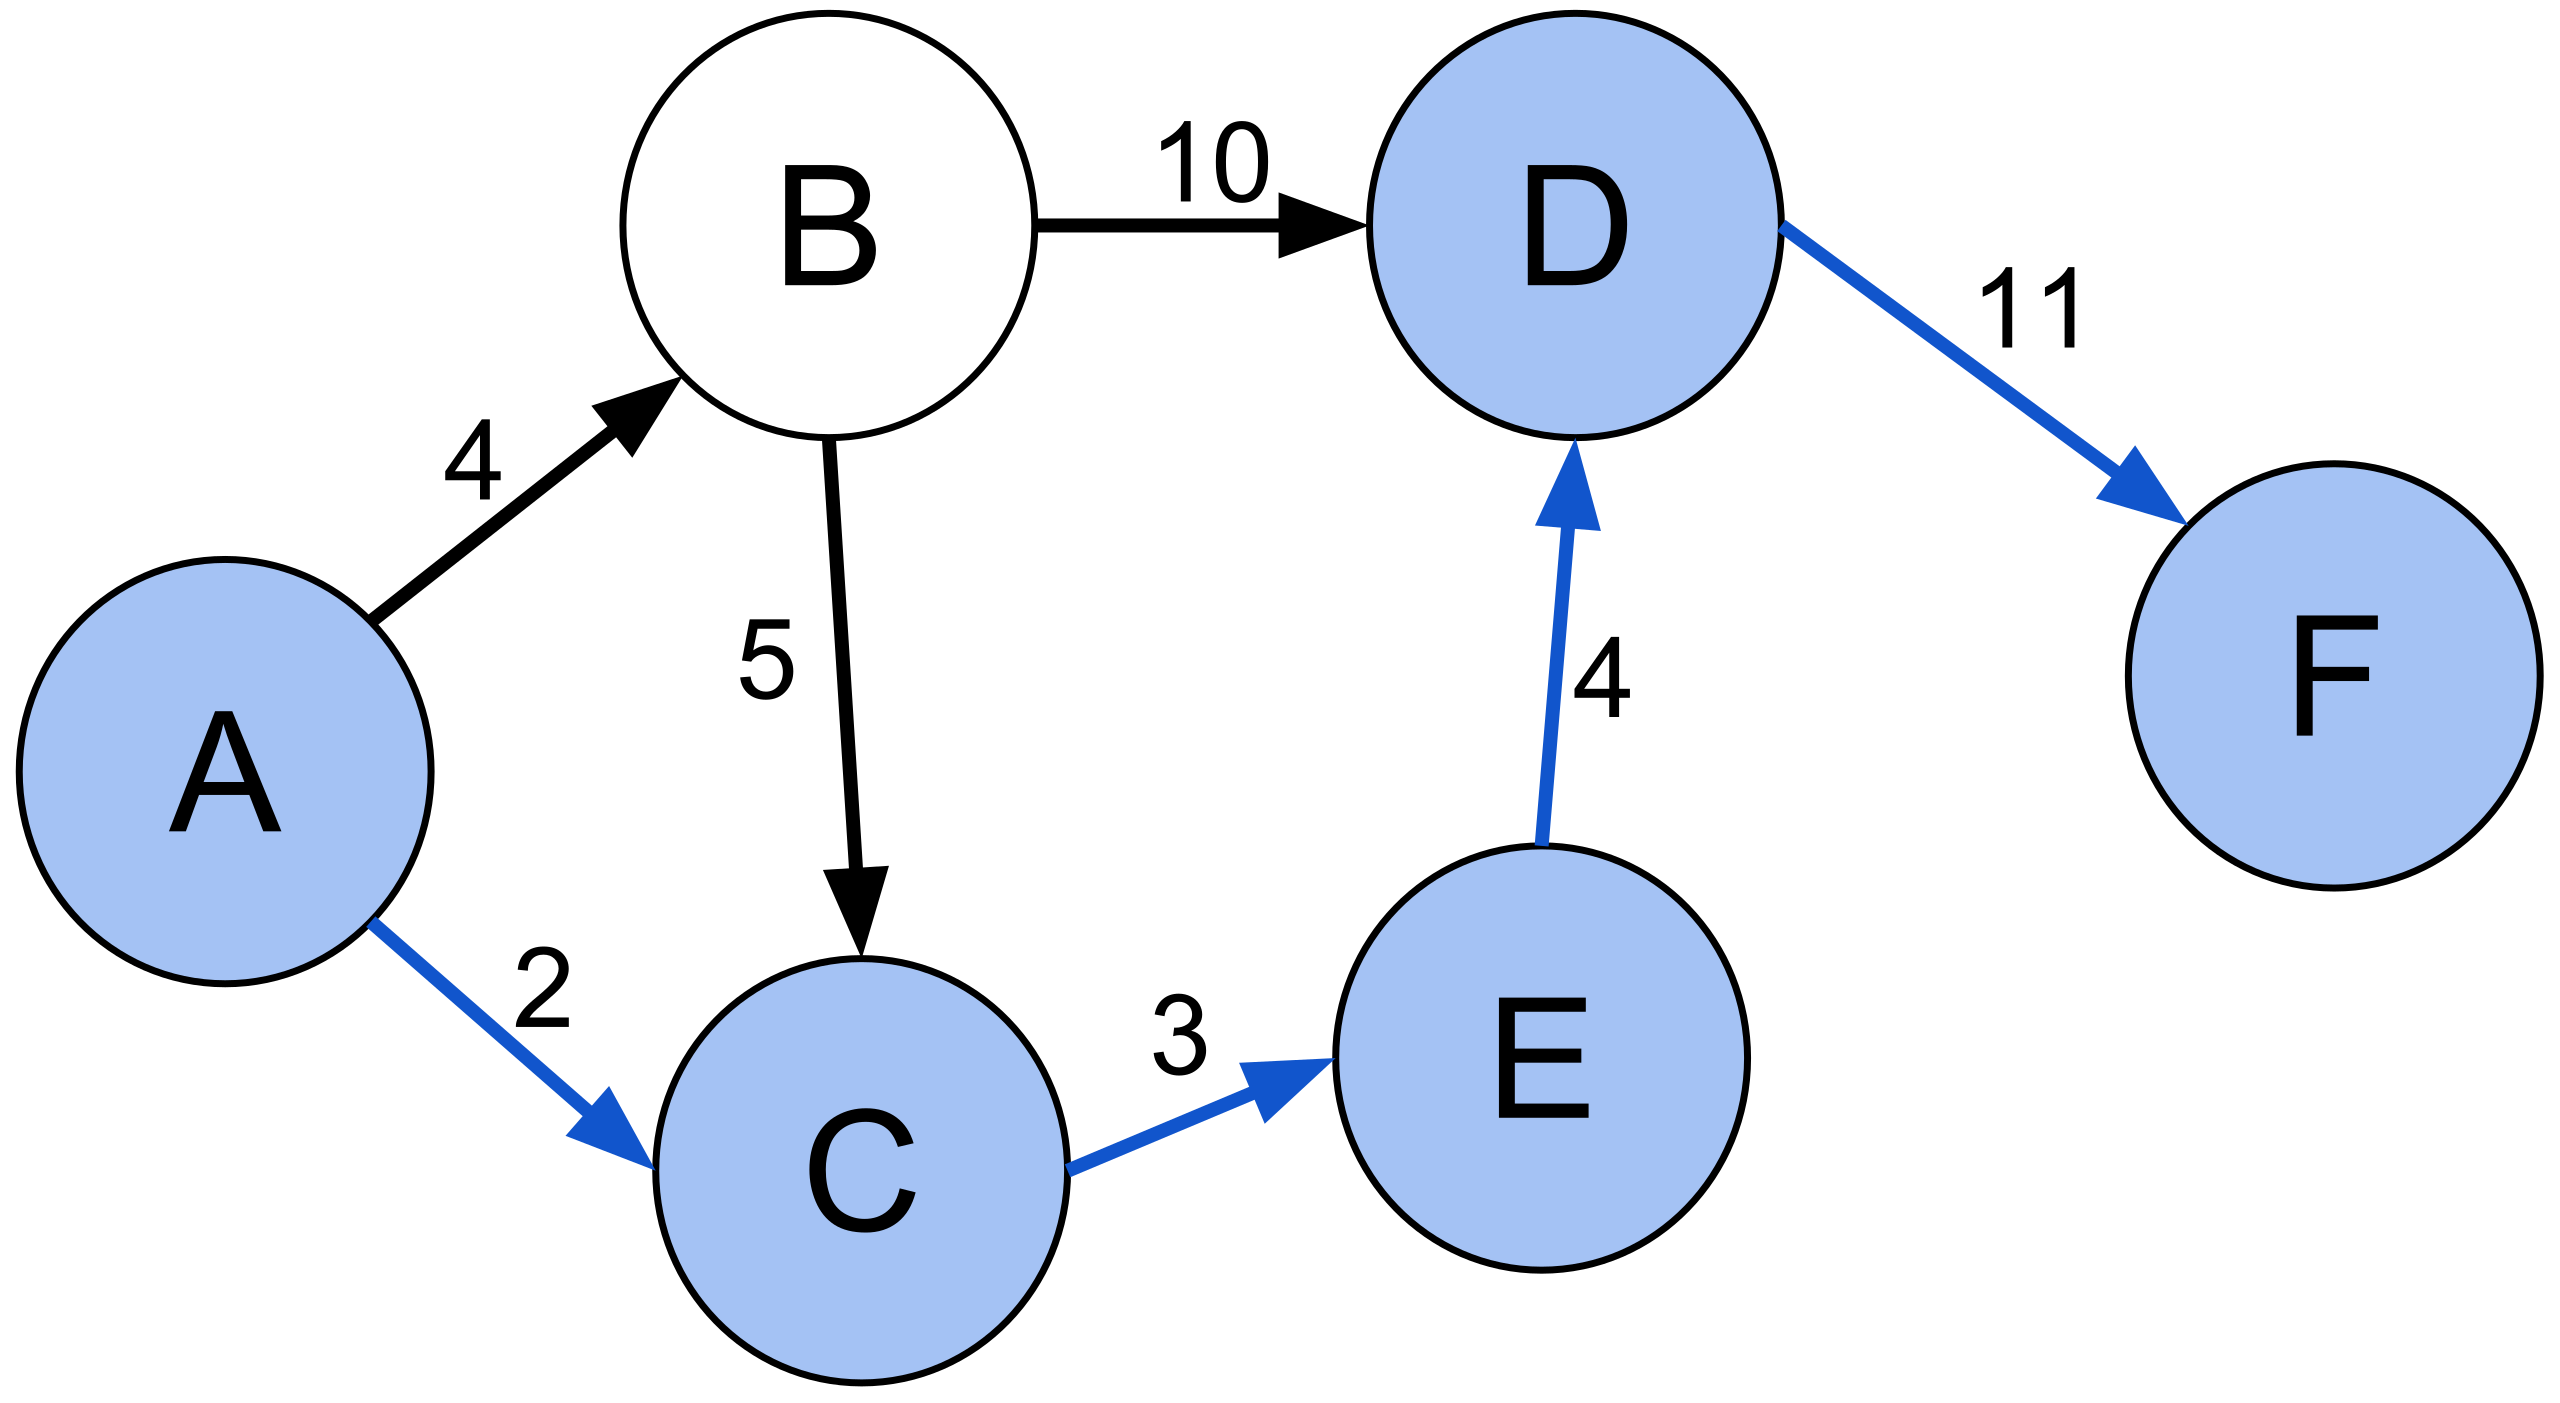
\includegraphics[width=0.6\textwidth]{shortest-path-wiki}
        \caption{%
            Korteste rute fra $A$ til $F$ er givet ved de blå kanter (fra
            Wikipedia)
        }
        \label{fig:shortest-path-wiki}
    \end{figure}
\end{frame}


\subsection{Pseudo-kode}

\begin{frame}{Pseudo-kode}

    Når vi arbejder algoritmer beskriver vi dem (typisk) i \alert{pseudo-kode}.
    Det vil sige kode, der ikke har samme rigide regler og strukturer, som C,
    C++, Java, Python, etc.\ men som ligner disse sprog og bruger samme
    kontrolstrukturer (loops, if/else og så videre).

    \medskip

    Målet er at beskrive \alert{tydeligt og koncist}, hvilke skridt der udføres
    i algoritmen --- hvordan vi går fra et \alert{input} til et \alert{output}.

\end{frame}

\begin{frame}{Pseudo-kode}{Eksempel: `Find element'}

    \begin{columns}
        \column{.5\textwidth}
        \begin{itemize}
            \item Gennemgå alle elementer i $A$ en af gangen og sammenlign med
                $a$
            \item Hvis vi finder $a$ i listen, gem det index i variablen
                $j$
            \item Når vi er færdige med hele sekvensen, returner $j$
        \end{itemize}

        \column{.5\textwidth}

        \fbox{%
            \begin{minipage}{.9\linewidth}
                \begin{codebox}
                    \Procname{$\proc{Find-Element}(A, a)$}
                    \li $j \gets 0$
                    \li \For $i \gets 1$ \To \attrib{A}{length} \Do
                    \li \If $A[i] \gets a$ \Then
                    \li $j \gets i$
                    \End
                    \End
                    \li \Return $j$
                \end{codebox}
            \end{minipage}
        }

    \end{columns}

\end{frame}

\begin{frame}{Pseudo-kode}{Eksempel: `Find element'}

    \begin{columns}
        \column{.5\textwidth}
        \begin{itemize}
            \item For pseudo-kode tænker vi ikke på software-problemer såsom:
                \begin{itemize}
                    \item Data-abstraktion
                    \item Modularitet
                    \item Fejlhåndtering
                    \item Testning
                \end{itemize}
            \item Vi kan endda også finde på at bruge tekst fremfor `kode'
        \end{itemize}

        \column{.5\textwidth}

        \fbox{%
            \begin{minipage}{.9\textwidth}
                \begin{codebox}
                    \Procname{$\proc{Find-Element}(A, a)$}
                    \li $j \gets 0$
                    \li \For $i \gets 1$ \To \attrib{A}{length} \Do
                        \li \If $A[i]$ and $a$ are the same \Do
                            \li $j \gets i$
                        \End
                    \End
                    \li \Return $j$
                \end{codebox}
            \end{minipage}
        }

    \end{columns}

\end{frame}

\begin{frame}{Pseudo-kode}
    At kunne læse, forstå og følge alle skridt i pseudo-kode er \alert{absolut
    nødvendigt} for at kunne klare sig godt i kurset og til eksamen.

    \pause
    \medskip

    Derfor kommer der træning i dette i dagens exercises.
\end{frame}

\section{Excercises}%

\begin{frame}{Excercises}{}
    Findes på Moodle --- arbejd i grupper --- spørg ENDELIG!

    \begin{figure}[h]
        \centering
        
\includegraphics[width=0.8\textwidth]{exercises}
    \end{figure}
\end{frame}


\section{Hvordan studerer man algoritmer?}

\begin{frame}{Hvordan studerer man algoritmer?}{Hvad er vi egentlig
    interesserede i?}

    I computervidenskab har vi massere af problemer, hvor vi kender vores
    udgangspunkt/input (f.eks.\ en usorteret liste) og vores ønskede mål/output
    (f.eks.\ en sorteret liste). Studiet af algoritmer handler om, hvordan vi
    bedst kommer fra inputtet til outputtet.

\end{frame}

\begin{frame}{Hvordan studerer man algoritmer?}{Hvad er vi egentlig
    interesserede i?}

    Kurset her har overordnet set 3 fokuspunkter:

    \pause
    \begin{itemize}
        \item Introduktion til klassiske algoritmiske problemer, løsninger og
            teknikker \looseness -1
            \begin{itemize}
                \item Sorteringsproblemet, shortest-path, look-up
                \item Datastrukturer, såsom heaps, binære søgetræer og grafer
                \item Divide-and-conquer, greedy algorithms, dynamic programming
            \end{itemize}
        \pause
        \medskip
        \item Korrekthed --- hvordan kan vi overbevise os selv om, at algoritmen
            virker, som forventet?
        \pause
        \medskip
        \item Kompleksitet
            \begin{itemize}
                \item Hvor meget \alert{tid} tager algoritmen?
                \item Hvor meget \alert{plads} (hukommelse) kræver algoritmen?
            \end{itemize}
    \end{itemize}

\end{frame}

\subsection{Korrekthed}

\begin{frame}{Korrekthed}

    \begin{definition}[Korrekthed]
        En algoritme er \alert{korrekt}, hvis den --- givet et korrekt input ---
        med garanti returnerer det korrekte output. Vi siger, at algoritmen
        \alert{løser} det givne `computational' problem.
    \end{definition}

    \pause
    Hvis din sorteringsalgoritme, f.eks., kun returnerer en korrekt sorteret
    liste, hvis inputtet ikke indeholder dupletter, så er algoritmen ikke
    korrekt --- medmindre det var en del af problemspecifikationen!
    
\end{frame}

\begin{frame}{Korrekthed}{Eksempel: `Find-Element'}
    \begin{description}
        \item[Input] En sekvens $A$ og et element $a$
        \item[Output] Det første index i $A$ hvor $a$ kan findes og 0, hvis ikke
            $a$ er i $A$
    \end{description}

    \pause
    \begin{columns}
        \column{.5\linewidth}

        \begin{codebox}
            \Procname{$\proc{Find-Element}(A, a)$}
            \li $j \gets 0$
            \li \For $i \gets 1$ \To \attrib{A}{length} \Do
                \li \If $A[i] \gets a$ \Then
                    \li $j \gets i$
                \End
            \End
            \li \Return $j$
        \end{codebox}

        \uncover<4->{Returnerer \alert{det sidste} index, hvor $a$ optræder.}

        \column{.5\linewidth}

        \begin{codebox}
            \Procname{$\proc{Find-Element-v2}(A, a)$}
            \li $j \gets \attrib{A}{length}$
            \li \While $i > 0$ \Do
                \li \If $A[i] = a$ \Then
                    \li $j \gets i$
                \End
                \li $i = i - 1$
            \End
            \li \Return $j$
        \end{codebox}

        \uncover<5->{Returnerer \alert{det første} index, hvor $a$ optræder.}

    \end{columns}

    \medskip
    Er begge algoritmer korrekte? \uncover<3->{\alert{Nej!}}
\end{frame}

\begin{frame}{Korrekthed}{Eksempel: `Find-Element'}
    \begin{description}
        \item[Input] En sekvens $A$ og et element $a$
        \item[Output] Det \alert{sidste} index i $A$ hvor $a$ kan findes og 0,
            hvis ikke $a$ er i $A$
    \end{description}

    \pause
    \begin{columns}
        \column{.5\linewidth}

        \begin{codebox}
            \Procname{$\proc{Find-Element}(A, a)$}
            \li $j \gets 0$
            \li \For $i \gets 1$ \To \attrib{A}{length} \Do
                \li \If $A[i] \gets a$ \Then
                    \li $j \gets i$
                \End
            \End
            \li \Return $j$
        \end{codebox}

        \column{.5\linewidth}

        \begin{codebox}
            \Procname{$\proc{Find-Element-v3}(A, a)$}
            \li $i \gets \attrib{A}{length}$
            \li \While $i > 0$ and $A[i] \neq a$ \Then
                \li $i = i - 1$
            \End
            \li \Return $i$
        \end{codebox}

    \end{columns}

    \medskip
    Er begge algoritmer korrekte? \uncover<3->{\alert{Ja --- der findes mange
    korrekte algoritmer for at løse et problem.}}
\end{frame}

\begin{frame}{Korrekthed}{Formelle beviser}
    Næste gang ser vi på \alert{loop invarianter}, som er en måde at bevise, at
    en iterativ algoritme er korrekt.
\end{frame}

\subsection{Kompleksitet}

\begin{frame}{Kompleksitet}{Tid og plads}
    \begin{itemize}
        \item Computere er hurtige, men ikke uendeligt hurtige - og de har meget
            hukommelse, men ikke uendelig hukommelse
        \item Når vi taler om en algoritmes kompleksitet, så taler vi om den
            \alert{tid} (runtime) og \alert{plads} (space) den kræver
        \item Nogle gange (men IKKE altid!) er der et \alert{trade-off mellem
            kompleksiteten i tid og kompleksiteten i plads}
        \item Forskellige algoritmer kan løse det samme problem korrekt, men
            have meget forskellig kompleksitet
    \end{itemize}
\end{frame}

\begin{frame}{Kompleksitet}{Analyse}

        Når vi analyserer algoritmer, er der en række ting, vi er interesserede
        i:

        \pause
        \begin{itemize}
            \item Forudsige performance
                \begin{itemize}
                    \item Hvor lang tid/meget plads kræver min algoritme?
                    \item Er det overhovedet muligt at løse problemet med den
                        tid og den plads, jeg har til rådighed?
                \end{itemize}
                \pause
            \item Sammenligne algoritmer
                \begin{itemize}
                    \item Hvilken algoritme er bedst i en given situation?
                \end{itemize}
                \pause
            \item Give garantier
                \begin{itemize}
                    \item Algoritmen vil aldrig bruge \alert{mere} tid end X
                    \item Algoritmen kræver \alert{som minimum} X GB hukommelse
                \end{itemize}
        \end{itemize}
    
\end{frame}


\begin{frame}{Kompleksitet}{Analyse}
    Men\ldots Vi gider faktisk sjældent blive særligt konkrete (vi er jo
    videnskabsfolk, ikke praktikere!). Hvorfor ikke?

    \pause
    \begin{itemize}
        \item Den præcise tid en algoritme tager afhænger af mange ting:
            computerens hardware, programmeringssproget, mængden af andre
            processer igang, temperaturen i rummet og ikke mindst
            \alert{inputstørrelsen}
        \item Den præcise plads en algoritme kræver afhænger også af mange ting:
            computerarkitekturen, data repræsentationen og ikke mindst
            \alert{inputstørrelsen}
    \end{itemize}
\end{frame}

\begin{frame}{Kompleksitet}{Inputstørrelse}

    Hvad vi derfor går efter er, at bestemme kompleksiteten af en algoritme som
    \alert{en funktion af inputstørrelsen}. Det vil sige, hvordan udvikler tiden
    (og pladsen) sig, når størrelsen af inputtet stiger?

    \pause
    \begin{itemize}
        \item Husk, at en algoritme er bare en række \alert{operationer}
            (computational steps), der hver især tager en vis mængde tid at
            udføre (som afhænger af alle de der mærkelige ting, vi ikke har
            kontrol over)
        \item Vi siger derfor, at tiden som det tager en algoritme at køre,
            gives ved \alert{antallet af operationer}, den skal igennem for at
            generere sit output
        \item Ofte er inputtet en mængde af elementer (f.eks.\ en liste). Hvis
            der er $n$ elementer i inputtet siger vi, at inputstørrelsen er
            \alert{$n$}
        \item Når tiden er funktion af $n$ noterer vi den som $T(n)$
    \end{itemize}

\end{frame}

\begin{frame}{Kompleksitet}{Eksempel: `Find-Element'}
    Vi siger af hver linie $i$ er 1 operation og tager \alert{konstant} tid $c_i$.
    For afgøre tiden $T(n)$ skal vi tælle, hvor mange gange hver linie udføres:

    \begin{columns}
        \column{.5\textwidth}
        \begin{codebox}
            \Procname{$\proc{Find-Element}(A, a)$}
            \li $j \gets 0$
            \li \For $i \gets 1$ \To \attrib{A}{length} \Do 
                \li \If $A[i] \gets a$ \Then 
                    \li $j \gets i$
                \End
            \End
            \li \Return $j$
        \end{codebox}
        
        \column{.5\textwidth}
        \begin{codebox}
            \Procname{tid $\times$ antal gange}
            \zi \uncover<2->{{$c_1 \times 1$}}
            \zi \uncover<3->{{$c_2 \times n + 1$}}
            \zi \uncover<4->{{$c_3 \times n$}}
            \zi \uncover<5->{{$c_4 \times n_a$}}
            \zi \uncover<6->{{$c_5 \times 1$}}
        \end{codebox}
    \end{columns}

    \begin{align*}
        T(n)&= \uncover<2->{c_1} + \uncover<3->{c_2(n + 1)} + \uncover<4->{c_3
        \cdot n}
        + \uncover<5->{c_4 \cdot n_a} + \uncover<6->{c_5} \\
            &= \uncover<7->{n(c_2 + c_3) + c_4 \cdot n_a + c_1 + c_2 + c_5}
    \end{align*}

\end{frame}

\begin{frame}{Kompleksitet}{Analyse}

    \begin{itemize}
        \item Den \alert{eksakte} køretid for \proc{Find-Element} er dermed:
            $T(n) = n(c_2 + c_3) + c_4 \cdot n_a + c_1 + c_2 + c_5$
            \pause \medskip
        \item Men i \alert{best case}, hvor $a$ ikke er i $A$, er $n_a = 0$, så:
            $T(n) = n(c_2 + c_3) + c_1 + c_2 + c_5$
            \pause \medskip
        \item I \alert{worst case}, hvor alle elementer i $A$ er $a$, har vi:
            $T(n) = n(c_2 + c_3 + c_4) + c_1 + c_2 + c_5$
    \end{itemize}
    
\end{frame}

\begin{frame}{Kompleksitet}{Worst case analyse}

    \begin{columns}
        \column{.6\textwidth}
        \begin{itemize}
            \item Vi er (næsten altid) kun interesseret i en algoritmes worst
                case
            \item Dette gør analysen lettere --- vi behøver ikke forholde os
                til alle de forskellige måder inputtet kunne påvirke tiden (og
                pladsen), kun den værst tænkelige
            \item Det giver os en garanti for, at algoritmen aldrig vil tage
                længere tid end det
            \item For mange algoritmer er worst case næsten det samme som
                average case
        \end{itemize}

        \column{.4\textwidth}
        
\includegraphics[width=\linewidth]{worst-case}
    \end{columns}
    
\end{frame}

\begin{frame}{Kompleksitet}{Analyse}
    Nu gør vi noget frækt. \pause Som sagt behandler vi tiden hver enkelt
    operation tager som en konstant. Det vil sige, den ændrer sig ikke. En
    konstant plus en konstant er også en konstant. Derfor siger, at $c_2 + c_3 +
    c_4 = a$ (her er $a$ ikke vores element, men en ny konstant). Og vi siger at
    $c_1 + c_2 + c_5 = b$, hvor $b$ også er en ny konstant.

    \begin{equation*}
        T(n) = \only<-2>{(c_2 + c_3 + c_4)}\uncover<3->{a}n + \only<-3>{c_1 + c_2
        + c_5}\uncover<4->{b}
    \end{equation*}

    \uncover<5->{%
        \begin{block}{Lineær vækst}
            Bemærk at $T$ er en \alert{lineær} funktion af $n$ med den klassiske
            form $an + b$. Det vil sige, når $n$ vokser med 1 vokser $T(n)$ med $a$
            og når $n=0$ er $T(n) = b$.
        \end{block}
    }
\end{frame}

\begin{frame}{Kompleksitet}{Order of growth}
    Nu gør vi noget endnu mere frækt. \pause

    \begin{itemize}
        \item Vi har allerede abstraheret det konkrete tidsforbrug væk ved at
            introducere ukendte konstanter ($c_1, c_2, \ldots)$
            \pause
        \item Vi kan abstrahere endnu mere ved kun at kigge på \alert{order of
            growth}
            \pause
        \item Vi \alert{ignorerer konstanter} og ser kun på, om tiden udvikler
            sig \alert{lineært}, \alert{logaritmisk}, \alert{kubisk}, etc.\ med
            inputtet
            \pause
        \item For \proc{Find-Element} får vi dermed en worst case køretid
            \alert{$T(n) = O(n)$}
            \pause
        \item I næste forelæsning går vi dybere ind i forskellige notationer for
            køretid, såsom $O, \Theta, \Omega$
    \end{itemize}
    
\end{frame}

\begin{frame}{Opsamling}{Dagens temaer}
    \begin{itemize}
        \item Hvad er algoritmer? 
        \item Problemspecificering ved inputs og outputs
        \item Pseudo-kode til at beskrive algoritmer
        \item Algoritmers korrekthed
        \item Kompleksitet og worst case analyse
    \end{itemize}
\end{frame}

\begin{frame}{Tak for i dag!}{Flere exercises..}

    Den bedste måde ikke at snyde sig selv på er lave exercises!

    \begin{figure}[h]
        \centering
        
\includegraphics[width=0.8\textwidth]{exercises}
    \end{figure}
    
\end{frame}



\end{document}


